\documentclass[12pt, a4paper]{article}

% ── Paquetes ──────────────────────────────────────────────────────────────────
\usepackage[utf8]{inputenc}
\usepackage[T1]{fontenc}
\usepackage[spanish]{babel}
\usepackage{geometry}
\usepackage{amsmath, amssymb}
\usepackage{graphicx}
\usepackage{float}
\usepackage{booktabs}
\usepackage{hyperref}
\usepackage{fancyhdr}
\setlength{\headheight}{14pt}
\usepackage{titlesec}
\usepackage{parskip}

\usepackage{caption}
\usepackage{xcolor}
\usepackage{enumitem}

% ── Geometría ─────────────────────────────────────────────────────────────────
\geometry{
  top    = 2.5cm,
  bottom = 2.5cm,
  left   = 2.8cm,
  right  = 2.8cm
}

% ── Encabezado/pie ────────────────────────────────────────────────────────────
\pagestyle{fancy}
\fancyhf{}
\renewcommand{\headrulewidth}{0.4pt}
\fancyhead[L]{\small Ingeniería Metalúrgica}
\fancyhead[C]{\small Cálculo Avanzado}
\fancyhead[R]{\small Aplicaciones de series numéricas}
\fancyfoot[C]{\thepage}

% ── Formato de secciones ──────────────────────────────────────────────────────
\titleformat{\section}{\large\bfseries}{}{0em}{}[\titlerule]
\titleformat{\subsection}{\normalsize\bfseries}{}{0em}{}

% ── Hipervínculos ─────────────────────────────────────────────────────────────
\hypersetup{
  colorlinks = true,
  linkcolor  = blue!60!black,
  urlcolor   = blue!60!black,
  citecolor  = blue!60!black
}

% ──────────────────────────────────────────────────────────────────────────────
\begin{document}

% ── PORTADA CON TÍTULO ORIGINAL ───────────────────────────────────────────────
\begin{titlepage}
  \centering
  \vspace*{1.5cm}

  
\includegraphics[width=0.30\textwidth]{logo_utn.png}\\[1.5cm]

  {\LARGE\bfseries Aplicaciones de series numericas.\\[0.4em]
  Ganancia de cavidad LASER}\\[1.2cm]

  \rule{0.6\textwidth}{0.5pt}\\[1.0cm]

  \begin{tabular}{ll}
    \textbf{Cátedra:}  & Cálculo Avanzado \\[0.3em]
    \textbf{Carrera:}  & Ingeniería Metalúrgica \\[0.3em]
    \textbf{Alumno:}   & Darío Ricardo de Santiago Sasinka \\[0.3em]
    \textbf{Legajo:}   & 68456 \\[0.3em]
    \textbf{ORCID:}    & \href{https://orcid.org/0000-0002-7684-9532}{0000-0002-7684-9532} \\[0.3em]
    \textbf{Email:}    & \href{mailto:68456@metalurgica.frc.utn.edu.ar}{68456@metalurgica.frc.utn.edu.ar} \\[0.3em]
    \textbf{DOI:}      & \href{https://doi.org/10.13140/RG.2.2.29126.18241}{10.13140/RG.2.2.29126.18241} \\[0.3em]
    \textbf{Licencia:} & CC BY 4.0 \\
  \end{tabular}\\[1.5cm]

  {\large Universidad Tecnológica Nacional\\
  Facultad Regional Córdoba}\\[0.5cm]
  {\normalsize Septiembre 2020 — Revisión 2025}

  \vfill
\end{titlepage}

% ── RESUMEN Y PALABRAS CLAVE ──────────────────────────────────────────────────
\thispagestyle{plain}
\begin{abstract}
\noindent
Este trabajo explora la aplicación de series numéricas en el cálculo de la ganancia óptica
de una cavidad resonante láser. Se describe el principio de funcionamiento de los láseres,
su estructura física básica y los procesos de emisión espontánea, absorción y emisión
estimulada que gobiernan su operación. Se desarrolla una expresión analítica para la ganancia
umbral a partir del desarrollo en serie de Taylor de la función exponencial, considerando las
pérdidas por reflexión en los espejos de la cavidad. Se demuestra que la aproximación lineal
$e^{-2\alpha L} \approx 1 - 2\alpha L$ está justificada físicamente para la gran mayoría de
láseres industriales de alta reflectividad, y se analiza cuantitativamente el error de
truncamiento. El resultado obtenido,
$\alpha_c = (1 - R_1 R_2)/(2L)$,
es de utilidad directa en el diseño y optimización de láseres de potencia para procesos
metalúrgicos de manufactura avanzada, tales como el sinterizado selectivo por láser (SLM),
la fusión selectiva por láser (DMLS) y el mecanizado láser de alta precisión.

\medskip
\noindent\textbf{Palabras clave:} LASER, cavidad resonante, ganancia óptica, series de Taylor,
condición de umbral, procesos de manufactura láser, ingeniería metalúrgica.
\end{abstract}

\newpage
\tableofcontents
\newpage

% ══════════════════════════════════════════════════════════════════════════════
\section{Introducción}

El LASER (\textit{Light Amplification by Stimulated Emission of Radiation}) es un dispositivo
que opera bajo el principio de la emisión estimulada, usado para generar un haz de luz
coherente —tanto espacial como temporalmente— lo que permite producir haces monocromáticos
altamente concentrados y de gran intensidad.

Los dispositivos LASER tienen numerosas aplicaciones en la vida moderna: desde la reproducción
de audio en soportes ópticos (CD/DVD) hasta aplicaciones de energía nuclear en laboratorios
de fusión por confinamiento inercial. Sin embargo, el interés prioritario para la ingeniería
metalúrgica reside en su aplicación en procesos de manufactura avanzada:

\begin{itemize}[leftmargin=2em]
  \item \textbf{Mecanizado láser:} corte, soldadura y perforación de alta precisión.
  \item \textbf{Impresión 3D metálica:} sinterizado láser directo de metales (DMLS) y fusión
        selectiva por láser (SLM), procesos centrales de la manufactura aditiva industrial.
\end{itemize}

El presente trabajo se enfoca en el análisis matemático de uno de los componentes críticos
del láser: la \textbf{cavidad óptica resonante}. El objetivo es demostrar cómo las series
numéricas —específicamente el desarrollo en serie de Taylor— permiten modelar la condición
de umbral y calcular la ganancia de la cavidad. Este parámetro es fundamental para determinar
la energía mínima necesaria para la operación láser en aplicaciones industriales.

% ══════════════════════════════════════════════════════════════════════════════
\section{Componentes y Principio de Operación}

\subsection{Componentes básicos de un láser}

Un láser está constituido por tres componentes esenciales (Figura~\ref{fig:cavity_scheme}):

\begin{enumerate}[leftmargin=2em]
  \item \textbf{Cavidad óptica resonante:} conjunto de elementos ópticos, habitualmente dos
        espejos: uno de alta reflectancia ($\approx 100\,\%$) y otro parcialmente reflectante
        ($\approx 95\,\%$) que permite la salida del haz láser.
  \item \textbf{Medio activo:} sustancia —sólido, líquido o gas— situada dentro de la cavidad
        resonante donde se produce la emisión estimulada.
  \item \textbf{Sistema de bombeo:} mecanismo por el cual se aporta energía al medio activo;
        puede ser de origen lumínico, térmico, eléctrico o químico.
\end{enumerate}

\begin{figure}[H]
  \centering
  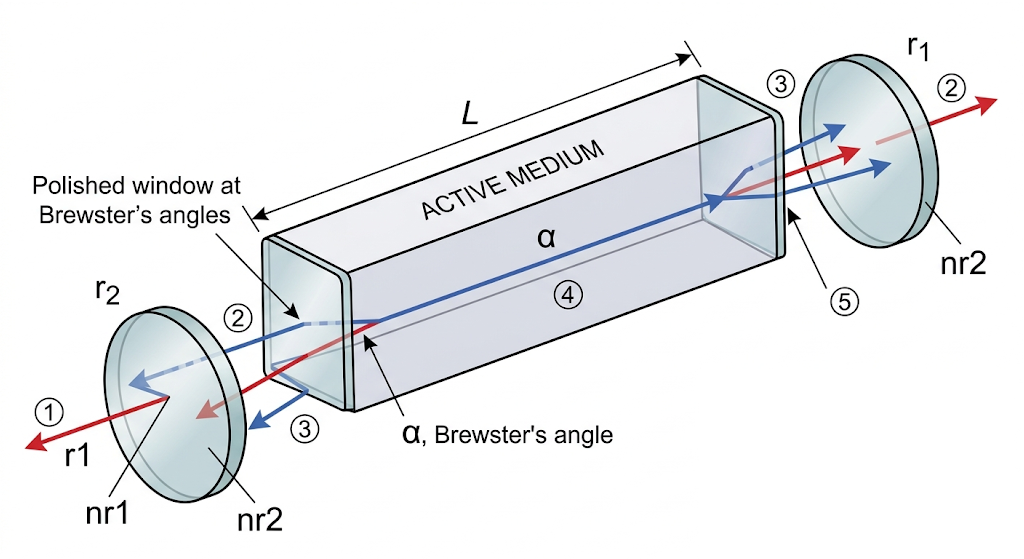
\includegraphics[width=0.88\textwidth]{cavity_scheme.png}
  \caption{Esquema de un láser de gas con ventanas de Brewster, medio activo central, espejo
    de alta reflectancia (izquierda) y espejo semitransparente de salida (derecha).}
  \label{fig:cavity_scheme}
\end{figure}

\subsection{Principios de operación — Mecánica cuántica del proceso}

Los electrones en los átomos se encuentran en niveles de energía discretos definidos por los
números cuánticos. En su nivel fundamental los electrones no absorben ni emiten energía.
La relación entre la energía de un fotón y la frecuencia de la radiación emitida está dada
por la relación de Planck-Einstein:
%
\begin{equation}
  \Delta E = h\,\nu
  \label{eq:planck}
\end{equation}
%
donde $\Delta E$ es la energía del fotón, $h$ es la constante de Planck
($h = 6{,}626 \times 10^{-34}$\,J$\cdot$s) y $\nu$ es la frecuencia de la radiación.

La Figura~\ref{fig:energy_levels} ilustra las transiciones energéticas posibles entre
niveles cuánticos discretos.

\begin{figure}[H]
  \centering
  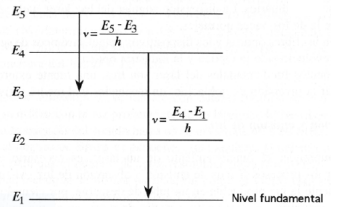
\includegraphics[width=0.58\textwidth]{energy_levels.png}
  \caption{Diagrama de niveles de energía. Las flechas representan transiciones electrónicas
    con emisión de fotones a las frecuencias correspondientes.}
  \label{fig:energy_levels}
\end{figure}

Cuando los electrones absorben energía saltan a un nivel superior; al decaer a un nivel
inferior emiten fotones. Normalmente en el medio activo, la mayoría de los átomos tienen sus
electrones en el estado fundamental, pero algunos átomos excitados emiten fotones
espontáneamente al volver a ese estado. Este proceso es aleatorio y los fotones emitidos
no son coherentes ni guardan ninguna relación de fase entre sí.

Cuando sobre un electrón en estado excitado incide una radiación de energía adecuada, el
átomo es \textit{estimulado} a emitir un fotón de la misma frecuencia y fase. Al sumarse
ambas radiaciones —la incidente y la emitida— se produce la \textbf{amplificación de la
radiación} (Figura~\ref{fig:emission_types}).

\begin{figure}[H]
  \centering
  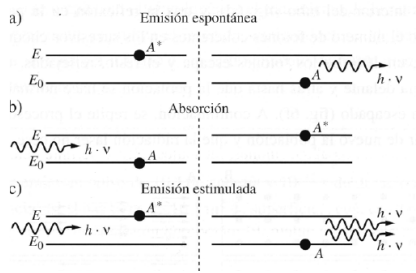
\includegraphics[width=0.72\textwidth]{emission_types.png}
  \caption{Los tres procesos radiativos: (a) emisión espontánea, (b) absorción y
    (c) emisión estimulada. Es este último el que sustenta la operación del láser.}
  \label{fig:emission_types}
\end{figure}

En condiciones normales la emisión estimulada es un efecto muy pequeño porque hay pocos
átomos en estado excitado. Para que un láser funcione, el medio activo debe contar con al
menos tres niveles energéticos y el sistema de bombeo debe lograr una
\textbf{inversión de población}: llevar la mayoría de los átomos al estado excitado, haciendo
muy probable la emisión estimulada (Figura~\ref{fig:population_inversion}).

\begin{figure}[H]
  \centering
  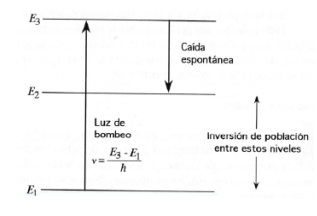
\includegraphics[width=0.52\textwidth]{population_inversion.png}
  \caption{Inversión de población en un sistema de tres niveles. La luz de bombeo promueve
    electrones de $E_1$ a $E_3$; la caída espontánea rápida a $E_2$ crea la inversión entre
    $E_2$ y $E_1$ necesaria para la emisión estimulada.}
  \label{fig:population_inversion}
\end{figure}

La cavidad resonante produce que los haces de luz se reflejen rebotando dentro de ella,
generando la emisión estimulada en fase en pulsos sintonizados a la longitud $L$ de la
cavidad (Figura~\ref{fig:cavity_resonant}).

\begin{figure}[H]
  \centering
  \includegraphics[width=0.88\textwidth]{cavidad_resonante.png}
  \caption{Cavidad resonante Fabry-Pérot. El haz recorre trayectorias de ida y vuelta
    ($1 \to 2 \to 3 \to 4 \to 5$) amplificándose en cada pasada a través del medio activo.
    $R_1$: espejo posterior de alta reflectancia; $R_2$: acoplador de salida semitransparente.}
  \label{fig:cavity_resonant}
\end{figure}

% ══════════════════════════════════════════════════════════════════════════════
\section{Condición de Umbral de la Cavidad}

La \textbf{condición de umbral} es el punto crítico en el que la ganancia de luz dentro de
la cavidad iguala exactamente las pérdidas, permitiendo que el láser comience a oscilar de
manera sostenida. Para establecerla, se definen las siguientes variables:

\begin{itemize}[leftmargin=2em]
  \item $\alpha$ \,[\,cm$^{-1}$]: ganancia por unidad de longitud en el medio activo.
  \item $L$ \,[cm]: longitud del material activo.
  \item $R_1,\, R_2$ \,(adimensionales, $0 < R_i \leq 1$): reflectividades de los dos espejos.
  \item $\phi$ \,[fotones/cm$^3$]: densidad de fotones en la cavidad.
\end{itemize}

Consideremos un haz que viaja paralelo al eje óptico. Al completar un viaje de \emph{ida y
vuelta} dentro de la cavidad, el haz experimenta:

\begin{enumerate}[leftmargin=2em]
  \item \textbf{Ganancia:} al atravesar el medio activo dos veces (distancia total $2L$), la
        densidad de fotones se multiplica por el factor de amplificación $e^{2\alpha L}$.
  \item \textbf{Pérdidas por reflexión:} al reflejarse en ambos espejos, la densidad se
        reduce en los factores $R_1$ y $R_2$.
\end{enumerate}

En el umbral, la densidad de fotones al inicio del ciclo $\phi_i$ debe ser igual a la
densidad al final del ciclo $\phi_f$:
%
\begin{equation}
  \phi_i \cdot e^{2\alpha L} \cdot R_1 \cdot R_2 = \phi_f
  \label{eq:umbral_completo}
\end{equation}
%
Dado que $\phi_i = \phi_f$ en el régimen estacionario del umbral, se simplifica a:
%
\begin{equation}
  e^{2\alpha L} \cdot R_1 \cdot R_2 = 1
  \quad\Longrightarrow\quad
  e^{-2\alpha L} = R_1 \cdot R_2
  \label{eq:umbral}
\end{equation}

Esta es la \textbf{ecuación de umbral exacta}: una ecuación trascendental que relaciona la
ganancia con las reflectividades de los espejos.

% ══════════════════════════════════════════════════════════════════════════════
\section{Desarrollo Matemático Mediante Series Numéricas}

\subsection{Expansión en serie de Taylor}

En el umbral, la ganancia $\alpha$ es una cantidad pequeña, por lo que el producto
$2\alpha L \ll 1$. Esto permite aproximar la función exponencial en la
ecuación~\eqref{eq:umbral} mediante su desarrollo en serie de Taylor (serie de Maclaurin)
alrededor del origen. La serie exponencial general es:
%
\begin{equation}
  e^{x} = \sum_{n=0}^{\infty} \frac{x^n}{n!}
         = 1 + x + \frac{x^2}{2!} + \frac{x^3}{3!} + \frac{x^4}{4!} + \cdots
\end{equation}
%
Sustituyendo $x = -2\alpha L$ en la ecuación de umbral~\eqref{eq:umbral}:
%
\begin{equation}
  e^{-2\alpha L}
  = \sum_{n=0}^{\infty} \frac{(-2\alpha L)^n}{n!}
  = 1 + (-2\alpha L) + \frac{(-2\alpha L)^2}{2!} + \frac{(-2\alpha L)^3}{3!} + \cdots
  = R_1 R_2
  \label{eq:serie_completa}
\end{equation}

La serie converge para todo valor de $\alpha L$, y en particular converge
absolutamente para $2\alpha L < 1$, condición que se cumple en láseres
industriales de alta reflectividad.

\subsection{Truncamiento de la serie — justificación física}

Dado que $\alpha$ es pequeño en el umbral, los términos de orden superior son mucho menores
que los primeros. Truncando la serie~\eqref{eq:serie_completa} después del término lineal:
%
\begin{equation}
  \boxed{e^{-2\alpha L} \approx 1 - 2\alpha L}
  \label{eq:aprox_lineal}
\end{equation}

Esta aproximación tiene una interpretación física precisa. Cada pasada por la cavidad
aporta una ganancia incremental pequeña; los términos de orden superior de la serie
corresponden a contribuciones de segundo, tercer y mayor orden de esas correcciones
acumuladas, que resultan despreciables cuando $2\alpha L \ll 1$.
Matemáticamente, el truncamiento equivale a la aproximación de primer orden
$e^{-x} \approx 1 - x$ para $|x| \ll 1$, justificada rigurosamente por el criterio
de convergencia de la serie de Taylor.

% ══════════════════════════════════════════════════════════════════════════════
\section{Cálculo de la Ganancia Característica}

Reemplazando la aproximación~\eqref{eq:aprox_lineal} en la condición de umbral:
%
\begin{equation}
  1 - 2\alpha_c L = R_1 R_2
\end{equation}

Despejando la \textbf{ganancia característica del oscilador} $\alpha_c$:
%
\begin{equation}
  \boxed{\alpha_c = \frac{1 - R_1 R_2}{2L}}
  \label{eq:ganancia}
\end{equation}

Este resultado es la expresión fundamental del trabajo. Es una fórmula analítica simple y
poderosa que permite calcular directamente la ganancia umbral mínima necesaria para que el
láser oscile, conocidos únicamente los parámetros geométricos y ópticos de la cavidad.

% ══════════════════════════════════════════════════════════════════════════════
\section{Análisis del Error de Truncamiento}

La aproximación lineal~\eqref{eq:aprox_lineal} introduce un error de truncamiento cuyo
término dominante es el término cuadrático de la serie:
%
\begin{equation}
  \varepsilon_{\rm trunc} \approx \frac{(2\alpha L)^2}{2}
  \label{eq:error}
\end{equation}

El \textit{error relativo} respecto al término lineal es de orden $\alpha L$:
%
\begin{equation}
  \varepsilon_{\rm rel} \approx \frac{(2\alpha L)^2/2}{2\alpha L} = \alpha L
\end{equation}

\subsection{Caso de alta reflectividad — láseres industriales típicos}

Para un láser de corte con $R_1 = 0{,}99$, $R_2 = 0{,}95$ y $L = 10$\,cm:

\begin{align}
  R_1 R_2 &= 0{,}9405 \\[4pt]
  \alpha_c &= \frac{1 - 0{,}9405}{2 \times 10} = \frac{0{,}0595}{20}
            = 2{,}975 \times 10^{-3}\;\text{cm}^{-1} \\[4pt]
  \varepsilon_{\rm trunc} &= \frac{(2 \times 2{,}975\times10^{-3} \times 10)^2}{2}
                           = \frac{(0{,}0595)^2}{2} \approx 1{,}77 \times 10^{-3}
\end{align}

El error cuadrático es tres órdenes de magnitud menor que el término lineal ($0{,}0595$).
La aproximación es excelente.

\subsection{Caso de baja reflectividad o cavidad muy larga}

Si $R_1 R_2 = 0{,}5$ o $L$ es muy grande, $\alpha$ crece y $2\alpha L$ deja de ser pequeño.
En este régimen la aproximación lineal pierde validez progresivamente. La
Tabla~\ref{tab:error} ilustra el comportamiento del error en función del producto
$2\alpha L$:

\begin{table}[H]
  \centering
  \caption{Error de la aproximación lineal en función de $x = 2\alpha L$.}
  \label{tab:error}
  \begin{tabular}{cccc}
    \toprule
    $x = 2\alpha L$ & $e^{-x}$ (exacto) & $1 - x$ (aprox.) & Error relativo \\
    \midrule
    0{,}05 & 0{,}9512 & 0{,}9500 & 0{,}13\% \\
    0{,}10 & 0{,}9048 & 0{,}9000 & 0{,}53\% \\
    0{,}20 & 0{,}8187 & 0{,}8000 & 2{,}28\% \\
    0{,}50 & 0{,}6065 & 0{,}5000 & 17{,}6\% \\
    1{,}00 & 0{,}3679 & 0{,}0000 & 100\%    \\
    \bottomrule
  \end{tabular}
\end{table}

Para valores de $x > 0{,}2$ se recomendaría incluir al menos el término cuadrático:
%
\begin{equation}
  e^{-2\alpha L} \approx 1 - 2\alpha L + \frac{(2\alpha L)^2}{2}
  \quad \Longrightarrow \quad
  \frac{(2\alpha_c L)^2}{2} - 2\alpha_c L + (1 - R_1 R_2) = 0
\end{equation}
%
que es una ecuación cuadrática en $\alpha_c$ con solución analítica exacta, o bien resolver
directamente la ecuación trascendental~\eqref{eq:umbral} numéricamente.

% ══════════════════════════════════════════════════════════════════════════════
\section{Discusión}

La expresión~\eqref{eq:ganancia} es el resultado central de este trabajo. Su derivación
conecta de manera directa el \textbf{cálculo avanzado} —la teoría de series de Taylor—
con un parámetro de diseño concreto en ingeniería de dispositivos láser.

Desde la perspectiva del diseño industrial:

\begin{itemize}[leftmargin=2em]
  \item La fórmula permite estimar rápidamente cuánta ganancia debe proporcionar el medio
        activo para que el láser supere el umbral, sin necesidad de resolver
        ecuaciones trascendentales.
  \item Los valores de $R_1$ y $R_2$ son parámetros de diseño controlables (calidad de los
        recubrimientos de los espejos), mientras que $L$ es un parámetro geométrico de la
        cavidad. La ganancia $\alpha_c$ requerida orienta la elección del medio activo
        (densidad de dopaje, longitud de amplificación).
  \item En procesos SLM/DMLS, donde se requiere alta densidad de potencia, se prefieren
        cavidades cortas con espejos de alta reflectividad, lo que mantiene $2\alpha L$
        pequeño y valida la aproximación lineal.
\end{itemize}

La convergencia de la serie y la validez de la aproximación lineal quedan justificadas
por las condiciones operativas típicas de alta reflectividad
($R_1 R_2 \gtrsim 0{,}9$, $x = 2\alpha L \lesssim 0{,}1$), donde el error es inferior
al 0{,}5\%.

% ══════════════════════════════════════════════════════════════════════════════
\section{Conclusión}

En el presente trabajo se ha demostrado la aplicación directa de las series numéricas
—específicamente la serie de Taylor— en un problema fundamental de la ingeniería láser:
el cálculo de la ganancia de una cavidad resonante.

Partiendo de la condición física de umbral para la densidad de fotones, se llegó a la
ecuación trascendental $e^{-2\alpha L} = R_1 R_2$. Mediante el desarrollo de esta
exponencial en serie de Maclaurin y el truncamiento al término lineal, se justificó
matemáticamente la aproximación $e^{-2\alpha L} \approx 1 - 2\alpha L$, y se obtuvo la
expresión analítica de la ganancia característica:
%
\begin{equation*}
  \alpha_c = \frac{1 - R_1 R_2}{2L}
\end{equation*}

El análisis del error de truncamiento confirma que la aproximación es excelente
(error $< 0{,}5\,\%$) para las condiciones operativas típicas de láseres de potencia
industrial, donde las reflectividades son muy altas ($R_1 \approx 100\,\%$,
$R_2 \approx 95\,\%$).

Se concluye que el cálculo avanzado, a través del uso de series numéricas, proporciona
herramientas esenciales para modelar y simplificar problemas complejos de la física de
dispositivos láser. Este modelado es fundamental para determinar la energía mínima
requerida para activar un láser de potencia industrial, optimizando así procesos
metalúrgicos de vanguardia como el sinterizado selectivo por láser y el mecanizado de
alta precisión.

% ══════════════════════════════════════════════════════════════════════════════
\section*{Referencias}

\begin{enumerate}[leftmargin=2em, label={[\arabic*]}]
  \item Saleh, B.E.A. \& Teich, M.C. (2007). \textit{Fundamentals of Photonics} (2nd ed.).
        Wiley-Interscience. Cap. 15.
  \item Svelto, O. (2010). \textit{Principles of Lasers} (5th ed.). Springer.
  \item Hecht, J. (2018). \textit{The Laser Guidebook} (2nd ed.). McGraw-Hill.
  \item Apostol, T.M. (1967). \textit{Calculus}, Vol. I. Blaisdell. Cap. 11 (Series de Taylor).
\end{enumerate}

\end{document}